\newpage
\section{Appendix}

Below we include a few areas where we could use some feedback.

\begin{enumerate}

	\item Is structural equivalence the right measure of the strength of a tie?
		\begin{enumerate}
			\item It has been convenient and readers will likely be familiar, but it also is not exactly what we are aiming for. If two states have very similar networks, then they are not necessarily strong allies, though the probability they are seems to increase. Another option is to fit a latent space model of alliance tie formation \citep{hoff2002} and then use the estimated Euclidean distances as a measure of tie strength.
			\item We could also construct multiple networks (alliances, trade, diplomatic ties, arms trade) and use similarity across the multiplex network to construct a multidimensional strength of tie measure.
		\end{enumerate}
	\item Canada's outsized contributions:
			\begin{figure}[H]
			\centering
				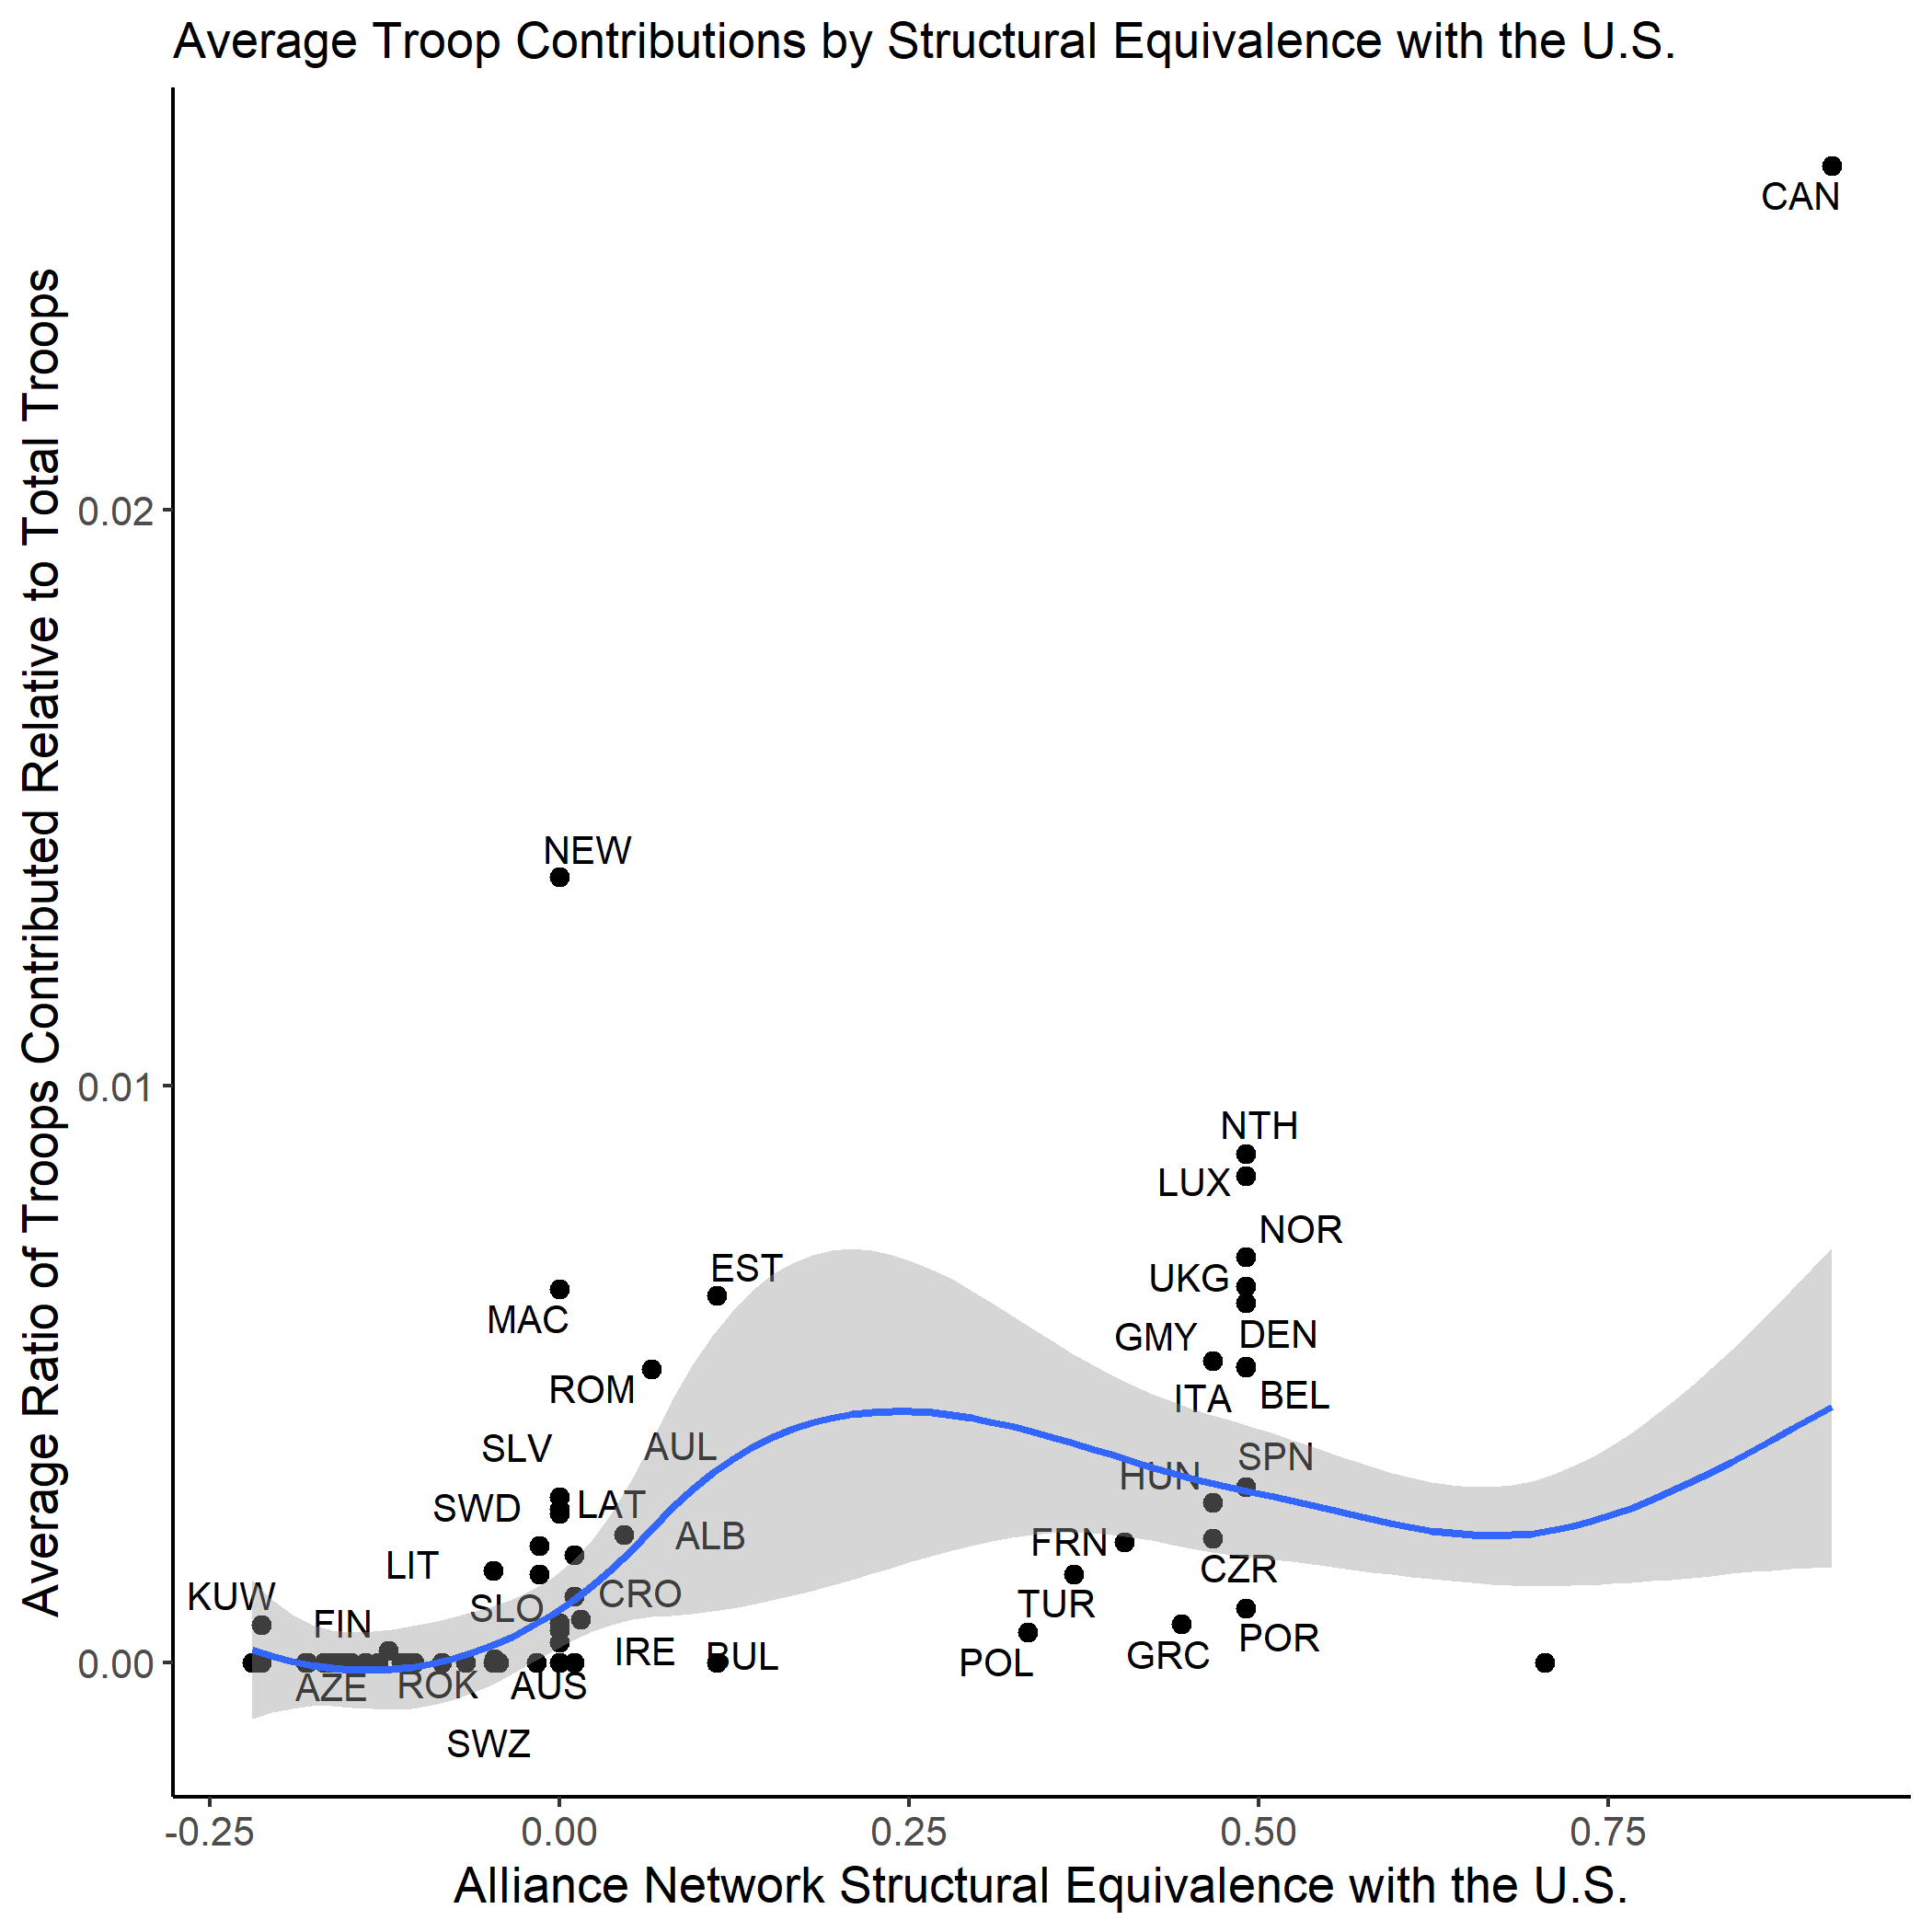
\includegraphics[width=0.55\textwidth]{figures/contributions_canada.png}
			\caption{Troop Ratio by Structural Equivalence with the United States}
			\label{fig:contr_sequiv_can}
			\end{figure}

		\begin{enumerate}
			\item Any thoughts on how to deal with this are appreciated.
		\end{enumerate}


	\item Next modeling steps:
	\begin{enumerate}
		\item Fit the model on 2001-2014 with Afghanistan, not just 2001-2005. But we need to deal with casualty aversion. Right now the plan is to just control for casualties on the right-hand side.
		\item We've received feedback to test the theory with the Iraq War. Though we haven't fit any models for Iraq yet, the data is almost ready and in identical format. So our plan is to finalize the empirical models for Afghanistan. treating it as a training set, and then we will test the models on Iraq. If the theory is accurate, then a model that captures the theory should have similar results -- not necessarily identical but similar in general relationship -- across conflicts. Iraq then will serve as a literal means of assessing out-of-sample performance.
	\end{enumerate}
\end{enumerate}
